\documentclass[11pt]{article}

\newcommand{\testName}{Mekanik prov \textbar{} MEKMEK01}
\usepackage{../prov}

\begin{document}
\raggedright{}
\section*{\testName}

\begin{center}
        \paddedfbox{
                Svara på frågorna som ställs genom att skriva svaret \textbf{på ett separat lösblad.} Du får inte ha formelblad. Du får inte heller använda miniräknare, men därför finns några förenklingar som du ska använda:
                \vspace{0.5em}
                \begin{itemize}[itemsep=0.5em]
                        \item Använd $g$ = \SI{10}{\meter/\second\squared} för enklare beräkning.
                        \item Om du tycker att beräkningen är för svår, avrunda inte, utan skriv ner hur du skulle göra om du hade en miniräknare.
                \end{itemize}
        }
\end{center}

\vspace{1em}

\begin{enumerate}[itemsep=0.5em]
        \item
              Skriv ditt namn: \underline{\hspace{5cm}} \textbf{(1p)}

        \item
              Vad betyder det att ett föremål är i jämvikt? \hrulefill{} \\
              \vspace{1em}
              \hrulefill{} \textbf{(1p)}

        \item
              \begin{minipage}[t]{0.6\textwidth}
                      Pelle väger 80 kg och lyfter en skivstång som väger 20 kg. Rita ut och beräkna de
                      krafter som verkar precis i toppen av lyftet, då han står helt stilla.

                      Betrakta Pelle och skivstången som en enhet, alltså rita inte ut krafter mellan händer och stång. \textbf{(3p)}
              \end{minipage}
              \hspace{2em}
              \begin{adjustbox}{valign=t}
                      \includesvg[width=6.5em]{pelle}
              \end{adjustbox}
        \item
              En bil som väger 2 ton kör i 90 km/h på motorvägen. De bromsande krafterna är totalt 5 000 N.
              \begin{enumerate}[label=\alph*)]
                      \item
                            Rita upp en skiss över bilen och krafterna som verkar på den. \textbf{(1p)}
                      \item
                            Hur mycket kraft behöver motorn ge för att bilen inte ska sakta ned? \textbf{(1p)}
                      \item
                            Hur mycket kraft måste vägen trycka på bilen för att bilen inte ska falla igenom marken? \textbf{(2p)}
              \end{enumerate}

        \item
              Pelle och hans lillasyster vill få gungbrädan i jämvikt. Pelle väger 80 kg och lillasystern väger 40 kg. Lillasystern sitter på brädans ände, vilket är 2 meter från mittpunkten. Hur långt från gungbrädans mittpunkt måste Pelle sitta? \textbf{(3p)}
              \begin{center}
                      \includesvg[width=25em]{gungbrada_prov}
              \end{center}

              \newpage
        \item
              I vilken/vilka av följande situationer visar sig \uline{mekanikens gyllene regel}?
              \begin{enumerate}[label=\alph*)]
                      \item En lång nyckel gör det enklare att dra åt en bult jämfört med en kort nyckel. \textbf{(1p)}
                      \item Tyngre föremål kräver mer kraft för att lyftas. \textbf{(1p)}
                      \item Det är jobbigare i stunden att cykla uppför en brant backe jämfört med en planare backe. \textbf{(1p)}
                      \item Ju längre sträcka du joggar, desto svårare blir det att fortsätta jogga. \textbf{(1p)}
              \end{enumerate}

        \item
              Vad är storleken på den resulterande kraften på bollen? Vad har den för vinkel mot horisontallinjen? Rita ut hur den resulterande kraften ser ut. \textbf{(2p)}
              \begin{center}
                      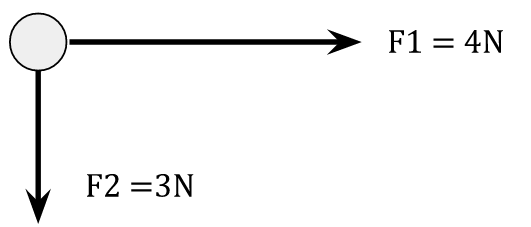
\includegraphics[width=25em]{kraft1.png}
              \end{center}

        \item
              \begin{minipage}[t]{0.6\textwidth}
                      En stege ligger stilla lutandes mot en vägg, den väger 10 kg. Det finns en friktionskraft mellan stegen och marken som är 50 N. Rita ut och beräkna fler krafter som kan tänkas finnas för att stegen ska vara i jämvikt. \textbf{(3p)}
              \end{minipage}
              \hspace{2em}
              \begin{adjustbox}{valign=t}
                      \includesvg[width=10em]{stege}
              \end{adjustbox}

        \item
              En bro som väger 15 ton ligger på två stödytor och är i jämvikt.  Avstånd mellan tyngdpunkt och vänster stödyta är 10 meter och avstånd mellan tyngdpunkt och höger stödyta är 5 meter.
              Beräkna hur mycket kraft varje stödyta tar upp. \textbf{(4p)}
              \begin{center}
                      \includesvg[width=0.8\textwidth]{bro}
              \end{center}


\end{enumerate}
\end{document}